\section{653 --- Two Sum IV - Input is a BST}
Given a Binary Search Tree and a target number, return \lstinline[language=C++, basicstyle=\small\ttfamily, keywordstyle=\bfseries\color{green!40!black}]|true| if there exist two elements in the BST such that their sum is equal to the given target.

\paragraph{Example 1:}

\begin{flushleft}
\textbf{Input}: 
\begin{figure}[H]
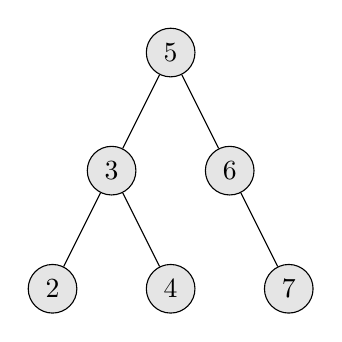
\begin{tikzpicture}
[every node/.style={draw, circle, fill=gray!20!, minimum size=5mm}]
\node{5}
child{node{3} child{node{2}} child{node{4}}}
child{node{6} child[missing] child{node{7}}};
\end{tikzpicture}
\end{figure}

\lstinline[language=C++, basicstyle=\small\ttfamily, keywordstyle=\bfseries\color{green!40!black}]|Target = 9|

\textbf{Output}: \lstinline[language=C++, basicstyle=\small\ttfamily, keywordstyle=\bfseries\color{green!40!black}]|true|
\end{flushleft}

 

\paragraph{Example 2:}

\textbf{Input}: 
\begin{figure}[H]
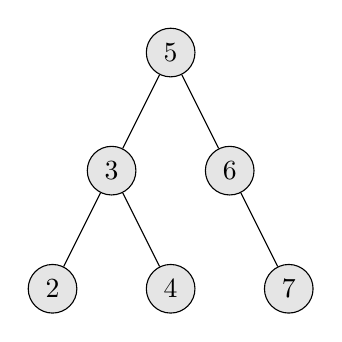
\begin{tikzpicture}
[every node/.style={draw, circle, fill=gray!20!, minimum size=5mm}]
\node{5}
child{node{3} child{node{2}} child{node{4}}}
child{node{6} child[missing] child{node{7}}};
\end{tikzpicture}
\end{figure}

\lstinline[language=C++, basicstyle=\small\ttfamily, keywordstyle=\bfseries\color{green!40!black}]|Target = 28|

\textbf{Output}: \lstinline[language=C++, basicstyle=\small\ttfamily, keywordstyle=\bfseries\color{green!40!black}]|false|

\subsection{Hash Set and Inorder Traverse}
We can traverse the tree by inorder approach, and make use of a hash set to store each node's value. When traversing, if the result of $k$ minus current node's value can be found in the hash set, it means there exists two numbers such that the sum of them is $k$.

\subsection{Convert To Sorted Array}
Since the given tree is a BST, the inorder traverse will give a sorted list (array). We can then use two pointers (indices) from both ends to check if there are two numbers whose sum is $k$.
